\chapter{Moving off Cardinal Planes}
\label{sec:non_orthogonal_pulleys}

We won't always be so lucky for our components to lie on a cardinal
(\emph{Front}, \emph{Right}, or \emph{Top}) plane. Next, lets move the cable run off the \emph{Right
  Plane}. Our goal is to end up at
  Figure~\ref{fig:completed-non-orthogonal}. One of the beauties of the 3D
sketch is that it will allow us to do this with very little modification to our part.

\begin{figure}[H]
\begin{center}
  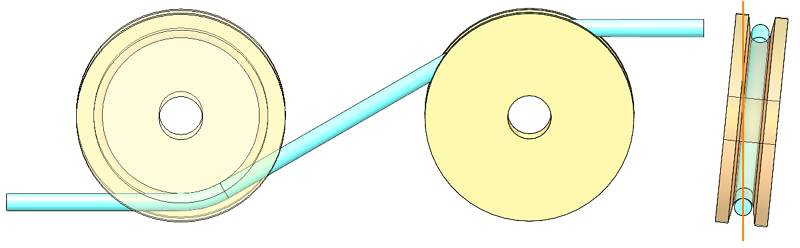
\includegraphics[width=5in]{images/figures/completed-non-orthogonal.png}
\end{center}
\caption{With a bit of editing to our 3D sketch, we'll be able to tilt our
  pulleys any way we please.
\label{fig:completed-non-orthogonal}}
\end{figure}

\section{Editing the 3D Sketch}

Edit \emph{3D Sketch 1} (which contains the geometry of our design). While we could
delete and re-draw lines and circles, this will break features within our Feature Tree.
Instead, we'll remove the relations that aren't working for us, and add new
relations in their place. If, when editing the sketch, you can't see the
relations, see Box~\ref{box:all_types}.

Remove the following relations and one dimension:

\begin{center}
\begin{tabular}{ccc}
  \hline
  \xrelation{On-Plane} & \emph{\sout{Circle 1}} & \emph{\sout{Front Plane}} \\
  \xrelation{On-Plane} & \emph{\sout{Circle 2}} & \emph{\sout{Front Plane}} \\
  \cadsymbol{Dimension} \sout{1.5''} & \emph{\sout{Line 1}} & \emph{\sout{Line 3}} \\
  \hline
\end{tabular}
\end{center}

Unfortunately, the \relation{On-Plane} relations show up with
\relation{Coincident} symbols, making them hard to find. The easiest way to
locate these relations is to select \emph{Circle~1}, then search the ``Existing
Relations'' list. Repeat for \emph{Circle~2}.

Our system is now ``Under Defined'', indicated by both the blue lines and the
\texttt{Under~Defined} at the bottom of the screen.
Drag \emph{Line 3} laterally in the positive X Direction. This will tilt both pulleys with respect to the cardinal planes.

\section{Controlling Cable Rise \& Run}
\label{sec:cable-rise-run}

Let's arbitrarily choose to separate \emph{Line 1} and \emph{Line 3} by \emph{0.1"} in
the \emph{X} direction and \emph{1"} in the \emph{Y} direction. The easiest way to do this
is to add three construction lines to connect \emph{Line 1} endpoint and
\emph{Line 3} endpoint, as in
Figure~\ref{fig:pulley-tilt-lines}. These construction lines should be
constrained \relation{Along-X}, \relation{Along-Y}, and \relation{Along-Z}, in
any order you prefer.

\begin{figure}[H]
\begin{center}
  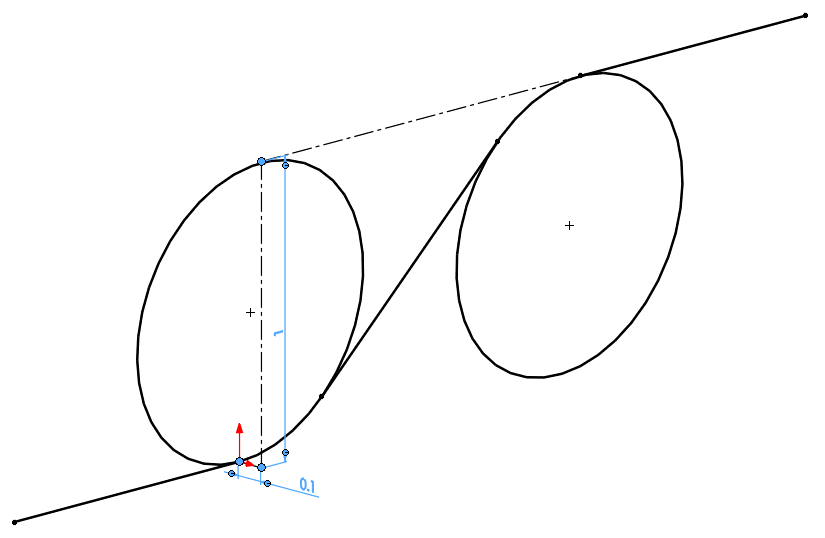
\includegraphics[width=5in]{images/figures/pulley-tilt-lines.png}
\end{center}
\caption{Add lines to control the separation between \emph{Line 1} and \emph{Line 3}.
Dimension the line that is \kode{Along~X} to \emph{0.1''} and the line that is
\kode{Along~Y} to \emph{1''}.
\label{fig:pulley-tilt-lines}}

\end{figure}

This should tilt both
Circles off the \emph{Right Plane}. Close the sketch
\cadsymbol{green-check}, and our part should rebuild
successfully. By keeping all sketch entities and only editing sketch relations,
our Feature Tree will happily rebuild without modification.

If you're like me, you ended up with one pulley tilting and the other staying
stubbornly upright, as in Figure~\ref{fig:pulley-not-tilted}. Take a moment to
consider why we've ended up here, and not where we wanted.

\begin{figure}[H]
\begin{center}
  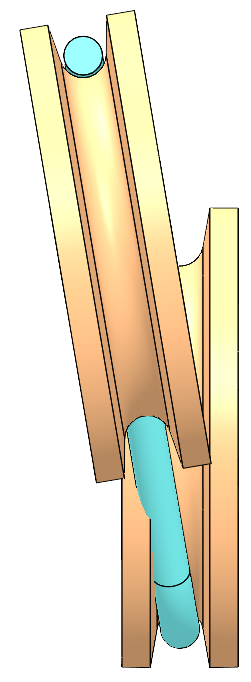
\includegraphics[height=3in]{images/figures/pulley-not-tilted.png}
\end{center}
\caption{While we wanted both pulleys to tilt off vertical, we only got one to move.
Where did we go wrong? \label{fig:pulley-not-tilted}}

\end{figure}

\subsubsection{An Easy (if Tedious) Fix}

The problem is that our pulley cross-section auto-defined with vertical and
horizontal relations. However, that is no longer (and never was) our design intent.
Instead, we want our pulley cross-section to be oriented with respect to our
cable path, which is no longer on the cardinal planes.

The way I fix this problem is to remove all the \relation{Horizontal} and
\relation{Vertical} relations from the pulley cross-section sketch and replace them with
\relation{Perpendicular} or \relation{Parallel} relations. The before-and-after
sketches are shown in Figure~\ref{fig:tilt-pulley-relations}. Be sure to make
the pulley axis \relation{Perpendicular} to \emph{Circle 1}.

Again, by modifying
relations, rather than deleting and replacing entities, we keep the Feature Tree
happy.

\begin{figure}[H]
\begin{center}
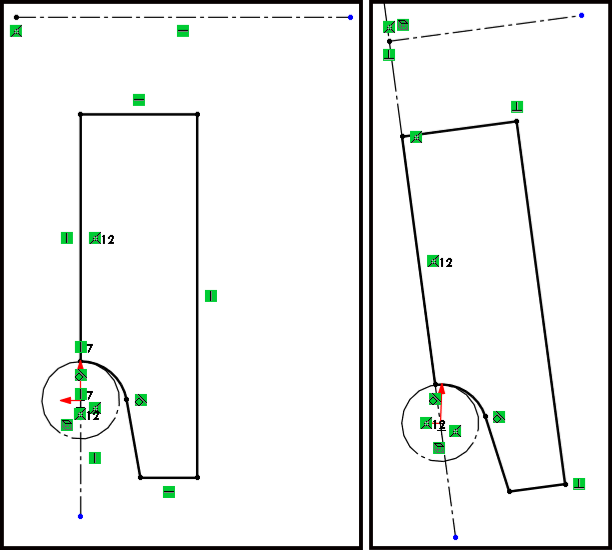
\includegraphics{images/figures/tilt-pulley-relations.png}
\end{center}
\caption{Sketch defined with horizontal and vertical relations (left) gives a vertical
  pulley. Redefine the sketch with relations perpendicular to \emph{Circle 1} to tilt
  \emph{Pulley 1}, which is what we want.
\label{fig:tilt-pulley-relations}}

\end{figure}

Now, when we rebuild \cadsymbol{green-check}, we find both pulleys happily
off-kilter (Figure~\ref{fig:completed-non-orthogonal2}). Lets relish this
moment, because in due time we'll put them back upright.

\begin{figure}[H]
\begin{center}
  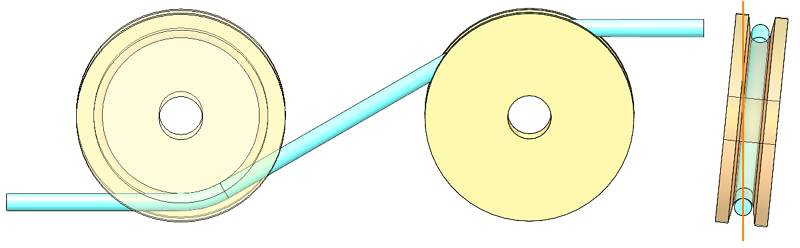
\includegraphics[width=5in]{images/figures/completed-non-orthogonal2.png}
\end{center}
\caption{The pulleys are again working as a team.
\label{fig:completed-non-orthogonal2}}

\end{figure}

\pagebreak

\begin{aside}
\label{box:all_types}
\heading{Hiding and Showing Types}

SolidWorks gives fine control over visibility of all things, including those that aren't
parts. One challenge to showing what you want is navigating the multiple ``On/Off'' switches that control
this visibility. As an example, let's show the pulley cross-section sketch,
which was already consumed by the \kode{Revolve} feature.

First, we must turn off \relation{Hide All Types}, found at the top of the
design window.

Next, within the \emph{Hide/Show Types} menu in the viewer window, we must turn on
``View Sketches'' \cadsymbol{Sketch}.

\begin{center}
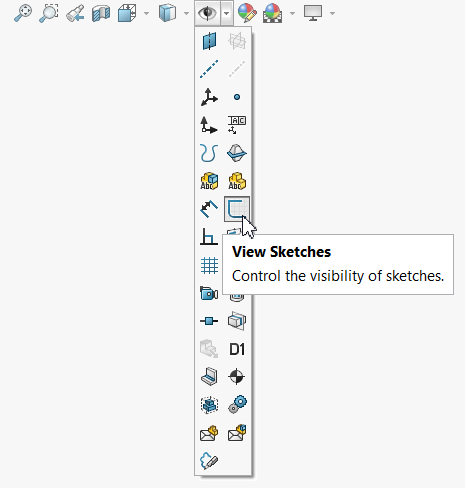
\includegraphics[height=3in]{images/figures/hide-show-menu.png}
\end{center}

Finally, we must ``Show'' \cadsymbol{show-eyeball} the
desired sketch within the Feature Tree. Visible sketches are indicated by a
colored sketch symbol \cadsymbol{Sketch}, whereas hidden ones are grey
\cadsymbol{Absorbed Sketch}.

\end{aside}
